\begin{frame}
    \frametitle{Научная новизна}
    \begin{itemize}
        \item Впервые были разработаны методы настройки оптического интерферометра на основе машинного обучения с подкреплением с использованием дискретного и непрерывного пространства действий
        \item Впервые создан программно-аппаратный комплекс настройки оптического интерферометра по изображениям с камеры основанный на машинном обучении с подкреплением
        \item Было выполнено оригинальное исследование применимости иерархического алгоритма сочетающего в себе машинное обучения с подкреплением и запрограммированное поведение для игры Nethack
        \item Был разработан оригинальный метод обучения стратегии для управления движением шагающего робота с заданной линейной и угловой скоростью
    \end{itemize}
\end{frame}
\note{
    Проговаривается вслух научная новизна
}

\begin{frame}
    \frametitle{Научная и практическая значимость}
    \begin{itemize}
        \item Применение предложенного в работе автоматизированного подхода к настройке оптического интерферометра позволит существенно ускорить проведение физических экспериментов и снизит необходимость в ручном труде
        \item Разработанные алгоритмы для управления виртуальными агентами затем могут быть применены в робототехнике, самоуправляемых автомобилях и виртуальных ассистентах
    \end{itemize}
\end{frame}
\note{
    Проговариваются вслух научная и практическая значимость
}

\begin{frame}
    \frametitle{Свидетельство о регистрации программы}
    \begin{figure}[h]
        \centering
        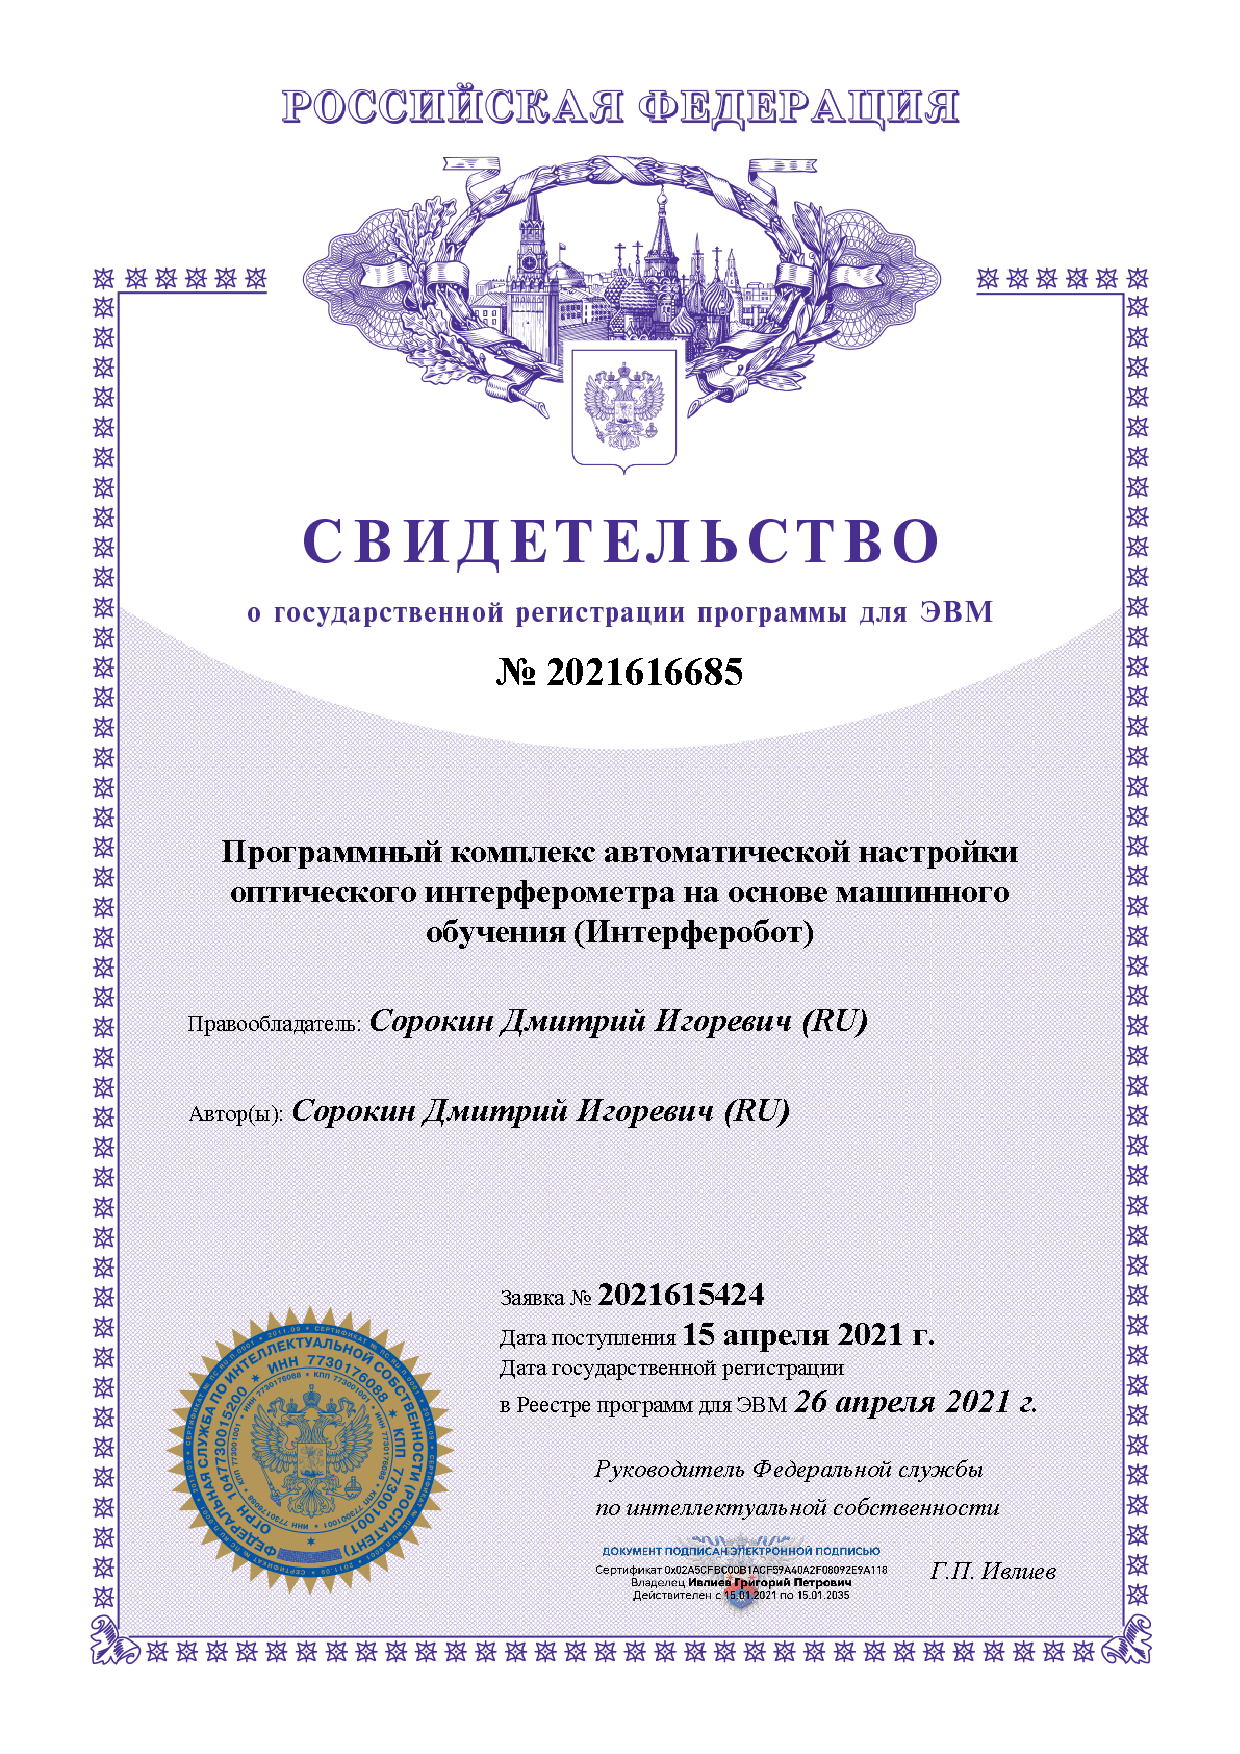
\includegraphics[height=0.7\textheight]{interferobot_rid.pdf}
    \end{figure}
\end{frame}
\note{
    Получено свидетельство о регистрации разработанной программы \textsc{Hello~world™}.
}

%\begin{frame}
%    \frametitle{Акт о внедрении}
%    \begin{figure}[h]
%        \centering
%        \fbox{
%            \begin{minipage}[t]{0.4\linewidth}
%                %\includegraphics[width=\linewidth]{implementation}
%            \end{minipage}
%        }
%    \end{figure}
%\end{frame}
%\note{
%    Получен акт о внедрении.
%}

\begin{frame} % публикации на одной странице
% \begin{frame}[t,allowframebreaks] % публикации на нескольких страницах
    \frametitle{Основные публикации}
    \nocite{vakbib1}%
    \nocite{vakbib2}%
    %
    %% authorwos
    \nocite{wosbib1}%
    %
    %% authorscopus
    \nocite{scbib1}%
    %
    %% authorconf
    \nocite{confbib1}%
    \nocite{confbib2}%
    \nocite{confbib3}%
    \nocite{confbib4}%
    %
    %% authorother
    \nocite{bib1}%
    \nocite{bib2}%
    \ifnumequal{\value{bibliosel}}{0}{
        \insertbiblioauthor
    }{
        \printbibliography%
    }
\end{frame}
\note{
    Результаты работы опубликованы в N печатных изданиях,
    в~т.\:ч. M реферируемых изданиях.
}

\begin{frame}
    \frametitle{Участие в конференциях}
    \begin{itemize}
        \item 34 международная конференции Neural Information Processing Systems (NeurIPS 2020) (доклад был отмечен как spotlight)
        \item 29 международная конференция по лазерной физике LPHYS’21
        \item 5 международная конференция Conference on Robot Learning (CoRL 2021)
        \item  35 международная конференция Neural Information Processing Systems (NeurIPS, Competition track 2021)
        \item Международная конференция по квантовым технологиям ICQT 2021
        \item Международная научно-техническая конференция Нейроинформатика 2022
    \end{itemize}
\end{frame}
\note{
    Работа была представлена на ряде конференций.
}

\begin{frame}[plain, noframenumbering] % последний слайд без оформления
    \begin{center}
        \Huge
        Спасибо за внимание!
    \end{center}
\end{frame}
